\documentclass[a4paper,twoside]{article}

\usepackage{epsfig}
\usepackage{subfigure}
\usepackage{calc}
\usepackage{amssymb}
\usepackage{amstext}
\usepackage{amsmath}
\usepackage{amsthm}
\usepackage{multicol}
\usepackage{pslatex}
\usepackage{apalike}
\usepackage{SCITEPRESS}
\usepackage[small]{caption}

\usepackage{siunitx}
\sisetup{
  locale = DE ,
  per-mode = symbol
}

\subfigtopskip=0pt
\subfigcapskip=0pt
\subfigbottomskip=0pt

\begin{document}

\title{EPE and Speed Adaptive Extended Kalman Filter for Vehicle Position and Attitude Estimation with Low Cost GNSS and IMU Sensors}

\author{\authorname{P. Balzer\sup{1}, T. Trautmann\sup{1} and O. Michler\sup{2}}
\affiliation{\sup{1}Laboratory of Vehicle Mechatronics,\\ Hochschule f\"ur Technik und Wirtschaft Dresden, Friedrich-List-Platz 1, 01069 Dresden, Germany}
\affiliation{\sup{2}Chair of Transport Systems Information Technology,\\Technische Universit\"at Dresden, Fakult\"at Verkehrswissenschaften "Friedrich List", 01062 Dresden, Germany}
\email{\{balzer, trautmann\}@htw-dresden.de, oliver.michler@tu-dresden.de}
}

\keywords{Multisensor Data Fusion, Adaptive, Extended Kalman Filter, Filter Tuning}

\abstract{This paper presents a novel approach for an adaptive Extended Kalman Filter (EKF), which is able to handle bad signal quality caused by shading or loss of Doppler Effect for low cost Global Navigation Satellite System (GNSS) receiver and Inertial Measurement Unit (IMU) sensors fused in a loosely coupled way. It uses the estimated  position error as well as the speed to calculate the standard deviation for the measurement uncertainty matrix of the Kalman Filter.
The filter is very easy to implement, because some conversions of the measurement, as well as the state variables, are made to reduce the complexity of the Jacobians, which are used in the EKF filter algorithm.
The filter implementation is tested within a simulation and with real data and shows significantly better performance, compared to a standard EKF.
The developed filter is running in realtime on an embedded device and is able to perform position and attitude estimation of a vehicle with low cost sensors.}

\onecolumn \maketitle \normalsize \vfill

\section{\uppercase{Introduction}}
\label{sec:introduction}

\noindent The Kalman Filter is widely used in a lot of applications, since R.E. Kalman introduced it in 1960 \cite{Kalman1960}. A vast number of papers have been published about the Kalman Filter and its special variations for special problems. A lot of them adressing problems about sensor fusion for unmanned autonomous vehicles, e.g. \cite{Penarrocha2010,Mourikis2007,Sun2010,Barczyk2011}. Implementations with adaptive calculation of the measurment uncertainty matrices $R$ and $Q$ are presented, e.g. \cite{Bistrovs2012}. Some of them deal with different driving situations (dynamic vs. standing) and using interactive multimodel fusion filtering, e.g. \cite{Toledo-Moreo2007,Stephen2001}. Some papers addressing problems with low cost sensors, e.g. \cite{Rosenberg2006,Toledo-Moreo2007,Kingston2004} and odometry
to supplement GNSS under signal masking conditions such as tree foliage and urban canyons, e.g. \cite{Stephen2001}.

Most of the papers using additional sensors like cameras \cite{Effertz2009,Holt2004}, wheel revolution sensors \cite{Stephen2001} or lidar sensors \cite{Holt2004} to get a better position estimation.
In this paper, we present a novel and very easy to implement adaptive EKF, which only uses low cost GNSS sensor and an intertial measurement unit (acceleration, rotation, magnetometer) to perform very well in dynamic situations and in rest position of a car.

No additional sensors nor a connection to the vehicle CAN is necessary, which recommends the filter for portable devices or Smartphones.

\section{\uppercase{Fundamentals}}

\subsection{Kalman Filter}

As introduced in \cite{Kalman1960}, the Bayesian tracking algorithm estimates the probability density function (PDF) of a systems state vector $x_k$, recursively. In one timestep $k$ the system state evolves with the state transition equation
\begin{equation}\label{statetransitionequation}
\boldsymbol{x}_{k+1}=g(\boldsymbol{x}_k, \boldsymbol{u}_k,\omega_k)
\end{equation}
to the next state. The noise $\omega$ is assumed to be zero mean multivariate Gaussian white noise with covariance $Q$.
\begin{equation}\omega_{k} \sim \mathcal{WN} (0, \boldsymbol{Q_k})\end{equation}
The control input $u$ drives the state.
The measurement function
\begin{equation}\label{measurementfunction}\boldsymbol{y}_{k}=h(\boldsymbol{x}_k,\nu_k)\end{equation} maps the measurements to the state vector with measurement noise $\nu$, which is as well assumed to be
\begin{equation}\nu_{k} \sim \mathcal{WN} (0, \boldsymbol{R_k})\end{equation}
with the measurement noise covariance matrix $R$.

\subsection{Uncertainty Matrices}

The matrices have different roles in the Kalman Filter. The matrix $Q$ models the uncertainty, which superimpose the system model. The matrix $R$ models the uncertainty associated with the measurements. The error covariance matrix $P$ is the matrix, which is recalculated in the prediction as well as in the correction step, by the Kalman filter itself. It shows the uncertainty of the state estimate as a function of time. Therefore, the values in $P$ should decrease over time.

\subsection{Linearization}

The Kalman Filter actually just works for linear states and measurements. Most of real life problems, like the one presented in this paper, are nonlinear, either on the dynamic or the measurement, or both.
The theory behind is, that a nonlinear state or measurement can be estimated by a Taylor approximation. The partial derivative of the state and the measurement with respect to state vector $x$ or control vector $u$ is well known as the Jacobian.

\begin{equation}J_{A} = \left . \frac{\partial g}{\partial \boldsymbol{x} } \right \vert _{\hat{\boldsymbol{x}}_{k},\boldsymbol{u}_{k}}\end{equation}

\begin{equation}J_{G} = \left . \frac{\partial g}{\partial \boldsymbol{u} } \right \vert _{\hat{\boldsymbol{x}}_{k},\boldsymbol{u}_{k}}\end{equation}

\begin{equation}J_{H} = \left . \frac{\partial h}{\partial \boldsymbol{x} } \right \vert _{\hat{\boldsymbol{x}}_{k},\boldsymbol{u}_{k}}\end{equation}

\subsection{Extended Kalman Filter}

Both, the Uncented and the Extended Kalman Filter perform evenly well on nonlinear states, but like St. Pierre et. al. in \cite{St-Pierre2004} pointed out, the Extended Kalman Filter is significantly more efficient in computational time. Depending on the complexity of the state transition function \eqref{statetransitionequation} and measurement function \eqref{measurementfunction}, the EKF is up to 22x faster \cite{St-Pierre2004}.

\begin{figure}[ht]
\centering
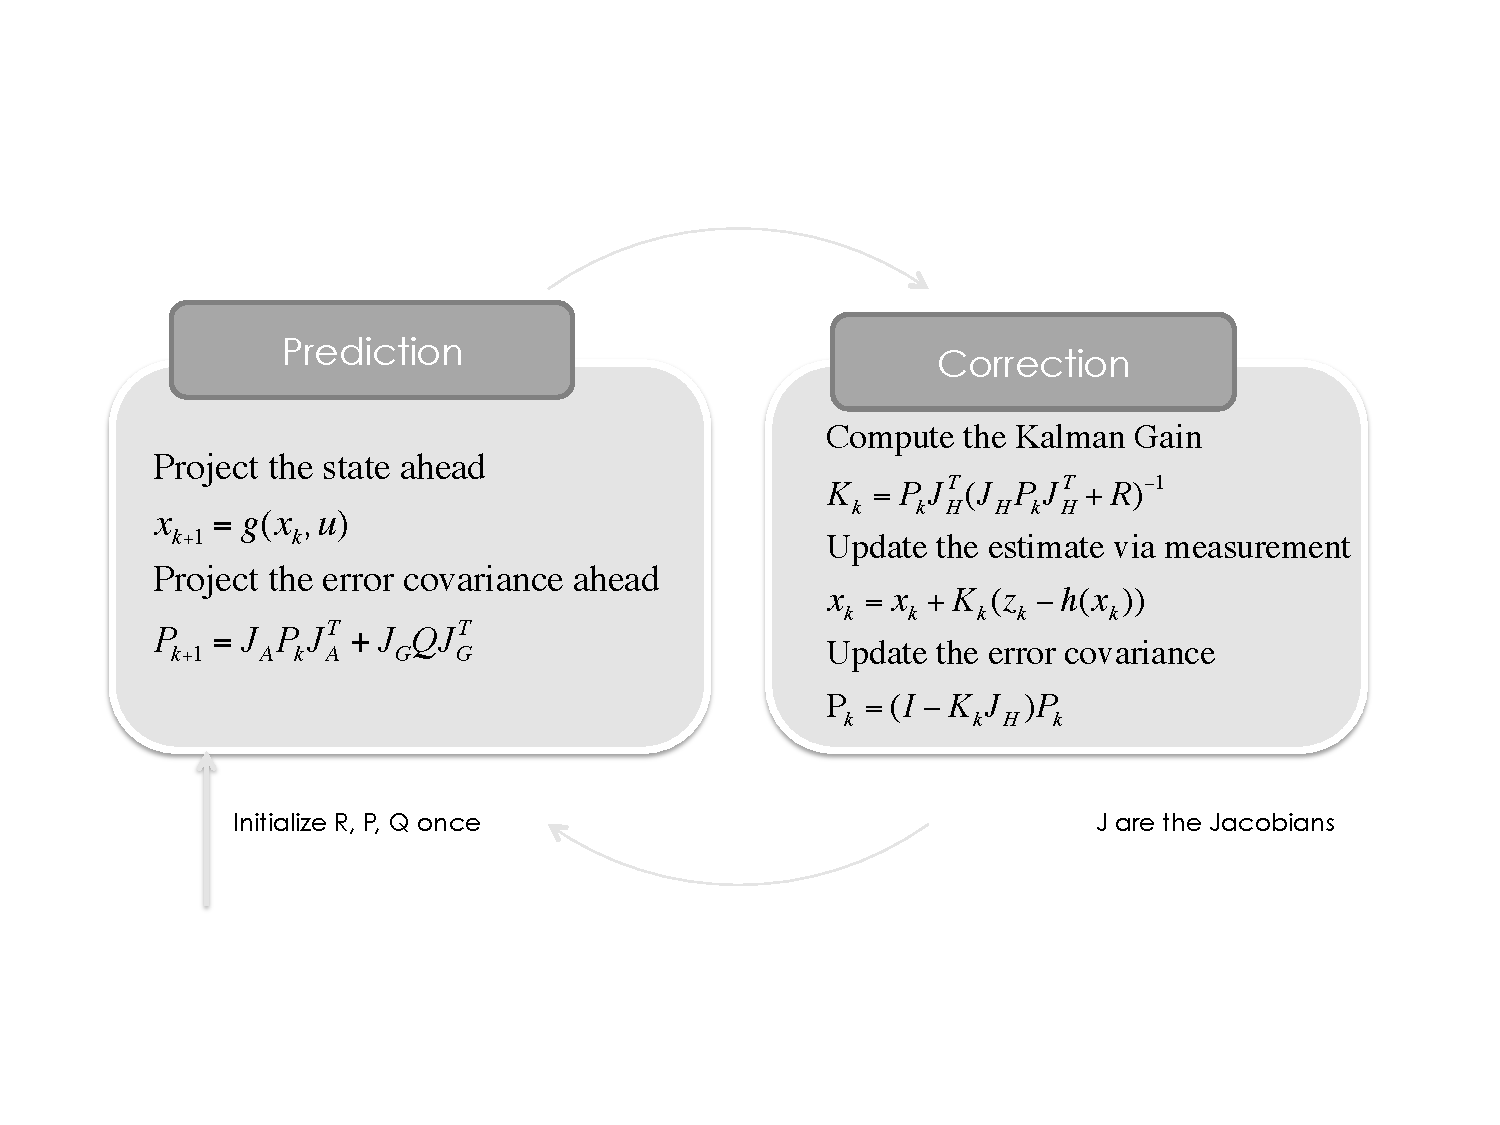
\includegraphics[width=3.0in]{images/Extended-Kalman-Filter-Step.pdf}
\caption{Extended Kalman Filter Step}
\label{EKF}
\end{figure}

Because the computational time is an important fact for real time state estimation, the EKF presented in this paper uses some calculations/conversions before the EKF itself, to reduce the complexity of the Jacobians, especially for the measurement function $h$.

\subsection{GNSS Position Accuracy}

In this paper, an adaptive extended Kalman Filter is introduced, which recalculates the measurement noise uncertainty for the position, based on the estimated position error ($EPE$), which is calculated by the GNSS receiver itself.

As \cite{Sharif} wrote, ``the EPE is a scalar indicating the precision of the receiver based on the deviation of the measurements from the mean of the measurement.''

For this reason, it cannot be used to determine a bias in the position measurement of the GNSS, but its relative error.

\begin{equation}EPE \sim \mathrm{HDOP} \cdot \mathrm{URA}(1 \sigma)\end{equation}

With $\text{HDOP}$ as the Horizontal Delution of Precision and $\text{URA}$ as the User Range Accuracy, which is a quantity that is transmitted in the navigation message and that is the predicted (not measured) statistical ranging accuracy.


\section{\uppercase{Extended Kalman Filter for CTRV dynamic with Attitude Estimation}}

The implemented EKF estimates following state vector $x_k$, which is well known as the constant turn rate and velocity (CTRV) vehicle model plus additionally roll and pitch estimation:

\begin{equation}\label{state}x_k= \left[ \begin{matrix} x\\y\\ v \\ \psi\\\phi\\\Theta \end{matrix}\right] = \left[ \begin{matrix} \text{Position x (GNSS)}\\ \text{Position y (GNSS)}\\ \text{Speed (GNSS)} \\ \text{Heading (GNSS)} \\ \text{Pitch (IMU)} \\ \text{Roll (IMU)} \end{matrix}\right]\end{equation}

As Schubert et. al. determined in \cite{Schubert2011}, "for ego motion estimation purposes which are characterized by a high update rate and the observability of $v$ and $\dot \psi$, model complexities beyond CTRV do not appear to be beneficial. However, the CTRV model shows its advantages as soon as a heading estimate is required."
The coordinate system is defined as shown in Fig.  \ref{KOS}.

\begin{figure}[ht]
\centering
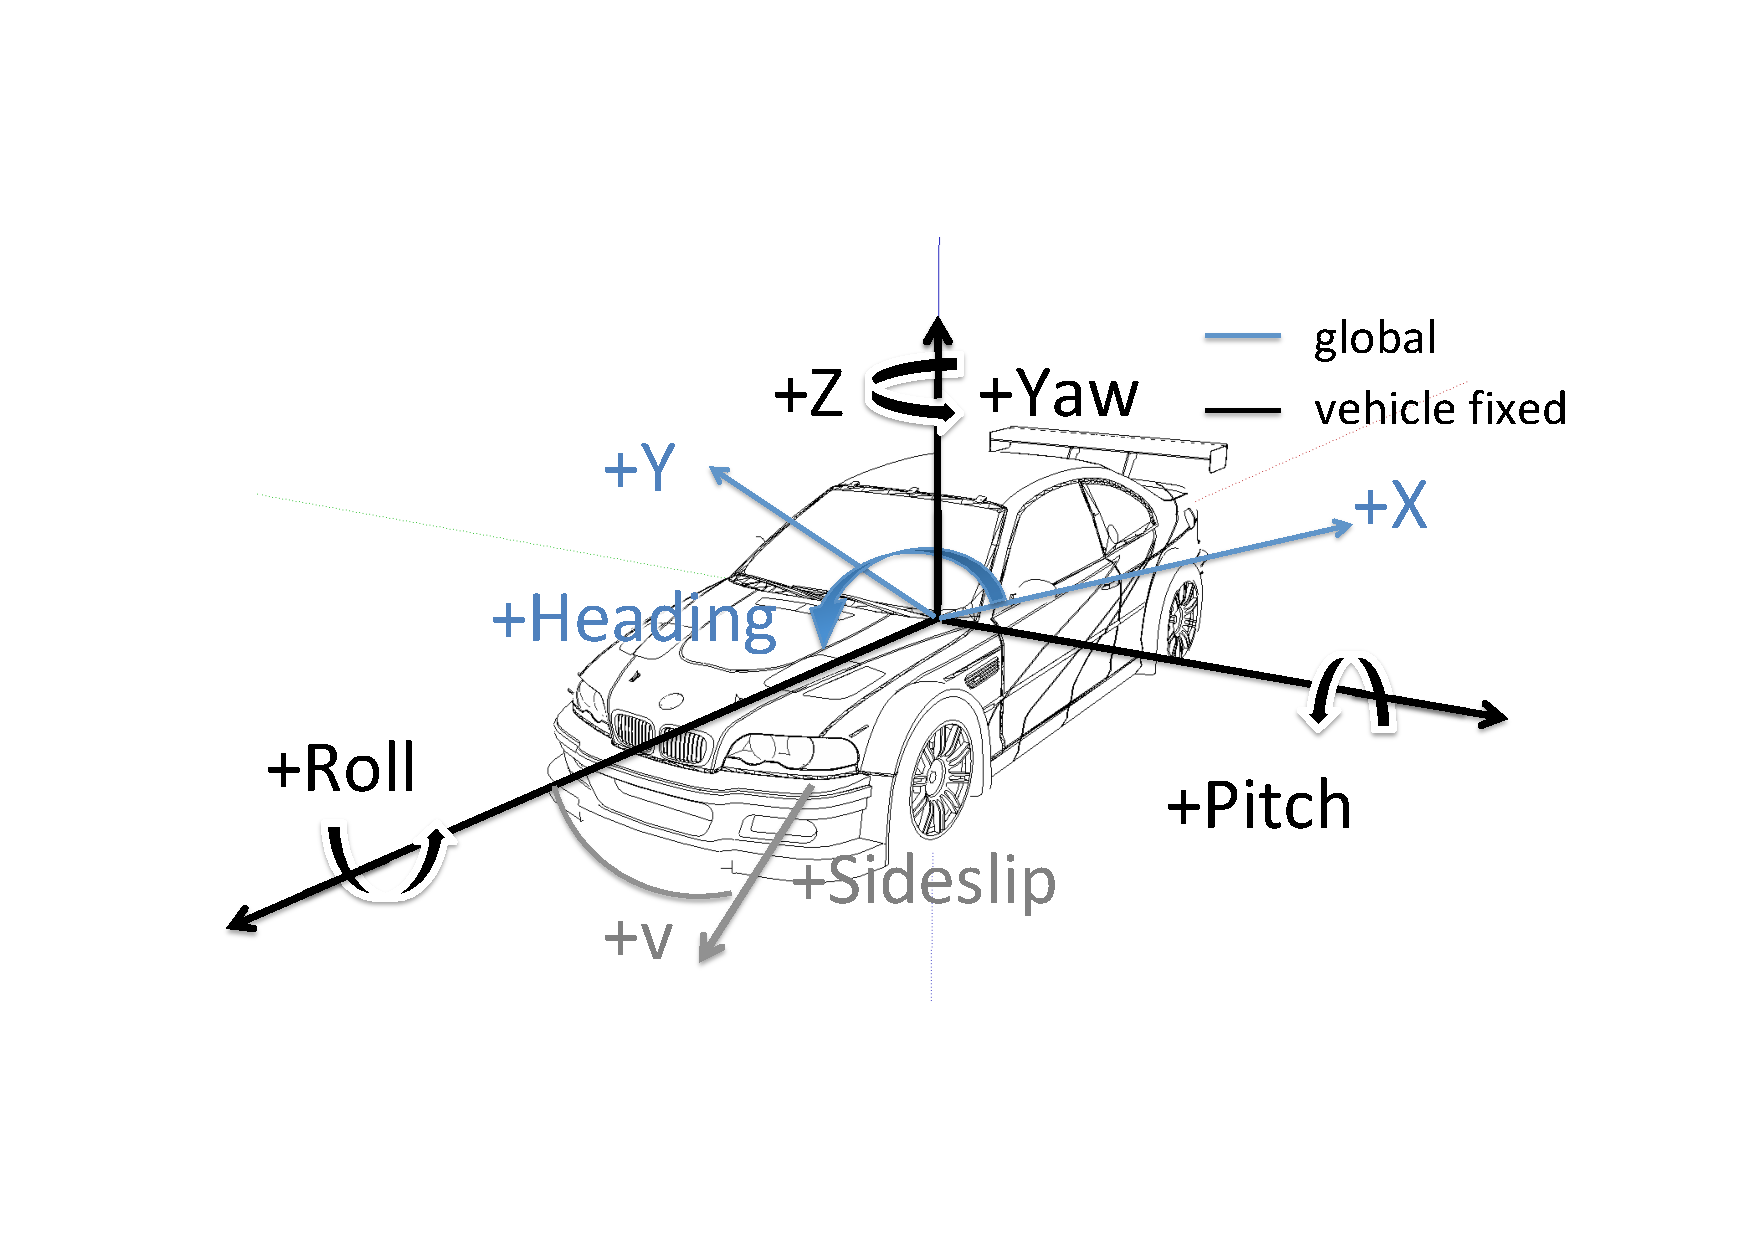
\includegraphics[width=2.6in]{images/Koordinatensystem-DIN70000.pdf}
\caption{Right hand coordinate system with z-axis to top}
\label{KOS}
\end{figure}

\subsection{Roll and Pitch Angle}

In \cite{Madgwick2010}, Madgwick presents an efficient orientation filter for inertial and inertial/magnetic sensor arrays. "The filter uses a quaternion representation, allowing accelerometer and magnetometer data to be used in an analytically derived and optimised gradient-descent algorithm to compute the direction of the gyroscope measurement error as a quaternion derivative.". The filter is implemented on the IMU and provides attitude information in quaternion representation in the global IMU coordinate system.

As mentioned there, the filter only estimates the correct attitude, if no external acceleration is actuating the vehicle. The calculated roll and pitch angles are actually just valid while standing still, not while accelerating/braking or cornering.

Madgwick recommended to adaptively choose convergence parameters, depending on absolute acceleration, influencing the IMU.

This paper lives this recommendation up and introduces an adaptively chosen weighting of roll and pitch angle, depending on the accelerations in lateral or longitudinal direction.

The roll and pitch angles, in vehicle coordinate system, are calculated with the quaternion ($Z_D=a-b\mathrm{i}_1-c\mathrm{i}_2-d\mathrm{i}_3$) output of the orientation filter \cite{Buchholz2013}.

\begin{equation}\label{rollangle}\phi = -\arcsin(2\cdot(a\cdot c - b \cdot d))\end{equation}
\begin{equation}\label{pitchangle}\theta = -\arctan\left(\frac{2\cdot(c\cdot d + a\cdot b)}{-(a^2-b^2-c^2+d^2)}\right)\end{equation}

\subsection{Position}

\noindent The position $x$ and $y$ is determined with a low cost GNSS receiver. The conversion between WGS84 $Lat$ and $Lon$ decimaldegrees to SI units is calculated as follows:
Assume the earth's radius at a specific altitude with $R=\SI{6378}{\kilo\metre}+alt$, then one degree of $Lon$ at $alt=\SI{0}{\metre}$ is
\begin{equation}arc = \cfrac{2 \pi\cdot (R+alt)}{\SI{360}{\degree}} =  \SI{111.32}{\kilo\metre\per\degree}\end{equation}

One degree $Lat$ is \SI{111.32}{\kilo\metre} only near the equator. If moving to the poles, the value decreases until it is \SI{0}{\kilo\metre} on North- or Southpole. Taking the $\cos$ of the $Lat$ provides the correct length reduction (see Fig. \ref{LonLatEquatorNorthpole}).

\begin{figure}[ht]
\centering
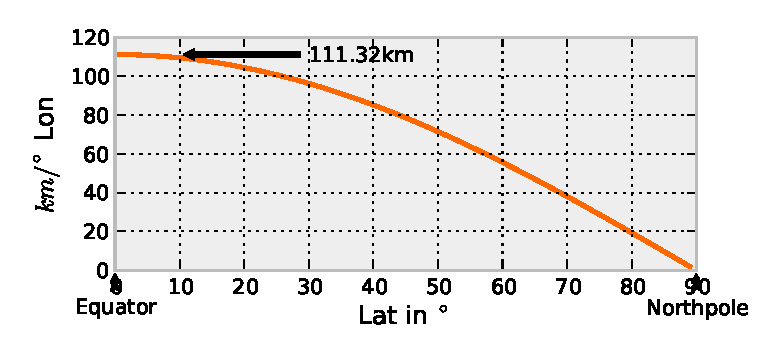
\includegraphics[width=3.0in]{images/Longitude-Cos-Latitude-Equator-Northpole}
\caption{Length of one degree of Longitude, depending on Latitude (WGS84)}
\label{LonLatEquatorNorthpole}
\end{figure}

\begin{equation}\label{deltax}\Delta x = arc\cdot\cos(Lat)\cdot\Delta Lon\end{equation}
\begin{equation}\label{deltay}\Delta y = arc\cdot\Delta Lat\end{equation}

With these equations the distance moved between two GNSS measurements can be calculated very accurate and additionally they simplify the state transition equations and the measurement function $h$, compared to other implementations, e.g. in \cite{Wender2008a}.

\subsection{State Control}

The longitudinal acceleration $a_x$, rollrate $\dot \Theta$, pitchrate $\dot \phi$ and the yawrate $\dot \psi$ are state control variables.

\begin{equation}\label{controlinput}u_k=\left[\begin{matrix}a_x & \dot\psi & \dot\phi & \dot\Theta \end{matrix}\right]^T\end{equation}

They are acquired by the IMU. The proposed filter could be used without any physical connection to the vehicle sensors (e.g. CAN-Bus) and therefore it is useful for mobile measurement systems. The state control vector $u$ consists only of values, acquired by the IMU, so the filter can run with high update rate in dead reckoning mode without GNSS information and the measurements from GNSS are used with lower update rate as correction.

\subsection{State Transition Function}

The state transition function $g(x_k, u_k)$ is defined with
\begin{equation}\label{statetransitionfunction}
x_{k+1}=\left[\begin{matrix}x + \frac{v}{\dot\psi} \left(- \sin{\left (\psi \right )} + \sin{\left (T \dot\psi + \psi \right )}\right)\\y + \frac{v}{\dot\psi} \left(\cos{\left (\psi \right )} - \cos{\left (T \dot\psi + \psi \right )}\right)\\T a_{x} + v\\T \dot\psi + \psi\\T \dot\phi + \phi\\T \dot\Theta + \Theta\end{matrix}\right]
\end{equation}

for $\dot \psi \neq 0$ and with $T$ as the time between two filtersteps. The Jacobians of the state transition with respect to the state and w.r.t. the control are listed in appendix.

\subsection{Process Noise Covariance Matrix Q}

As Kelly in \cite{Kelly1994} pointed out "a Kalman filter is a mathematical idealization that happens to be useful in practice. However, it is important to note that there is a big difference between an optimal estimate and an accurate estimate. In practical use, the uncertainty estimates take on the significance of relative weights of state estimates and measurements. So it is not so much important that uncertainty is absolutely correct as it is that it be relatively consistent across all models."

\begin{equation}Q=diag\label{Q}\left[\begin{matrix}\sigma_{a}^2 & \sigma_{{\dot\psi}}^2 & \sigma_{{\dot\phi}}^2 & \sigma_{{\dot\Theta}}^2 \end{matrix}\right]\end{equation}

Cross covariances resulting from deviation moments are assumed to be zero.

Assumptions for process noises for a vehicle model are suggested in \cite{Kelly1994}. The process noise is best described with the question, how much the state can be propagated in one timestep by expected movement of the vehicle. So the jerk expected for a car might be $\SI{300}{\metre\per\cubic\second}$ under normal circumstances, so the $\sigma_a \approx \dot a_\text{max}\cdot T$.

A typical maximal angular acceleration around vehicle z-axis might be $\SI{80}{\degree\per\square\second}$, which leads to a process noise of $\sigma_{\dot\psi} \approx \SI{80}{\degree\per\square\second} \cdot \frac{\pi}{180{,}0} \cdot T$.
The rotation around the pitch axis is much more dynamically, with typical angular accelerations of $\SI{200}{\degree\per\square\second}$ because of bumps and road surface quality. The angular acceleration around the roll axis is assumed to be $\SI{200}{\degree\per\square\second}$, too.

The process noises for a $\SI{50}{\hertz}$ filter are listed in Table \ref{processnoisetable}.

\begin{table}[ht]
%% increase table row spacing, adjust to taste
\renewcommand{\arraystretch}{1.3}
% if using array.sty, it might be a good idea to tweak the value of
% \extrarowheight as needed to properly center the text within the cells
\caption{Process Noise Standard Deviations}
\label{processnoisetable}
\centering
%% Some packages, such as MDW tools, offer better commands for making tables
%% than the plain LaTeX2e tabular which is used here.
\begin{tabular}{c l c}
\hline
Parameter & Decribtion & Value\\
\hline
$\sigma_a$ & Acceleration Process Noise & \SI{6.0}{\metre\per\square\second} \\
$\sigma_{\dot \psi}$ & Yawrate Process Noise & \SI{0.028}{\radian\per\second}\\
$\sigma_{\dot \phi}$ & Pitchrate Process Noise & \SI{0.070}{\radian\per\second}\\
$\sigma_{\dot \Theta}$ & Rollrate Process Noise & \SI{0.070}{\radian\per\second}\\
\hline
\end{tabular}
\end{table}

\subsection{Measurement Noise Covariance R}

The attitude estimation of the IMU filter \cite{Madgwick2010}, which is used as measurement for roll \eqref{rollangle} and pitch \eqref{pitchangle}, is only valid for quasistatic situations (which is acutally not valid for a moving vehicle), the standard deviation for the calculated attitude angles are adaptive to the accelerations $a_x$ for pitch and $a_y$ for roll.

The novel approach, presented in this paper, is the very easy to implement and fast to calculate elements of the measurement noise covariance matrix $R$.

\begin{equation}\label{R}R=diag\left[\begin{matrix}\sigma_{x}^2 & \sigma_{y}^2 & \sigma_{v}^2 & \sigma_{\psi}^2 & \sigma_{\phi}^2 & \sigma_{\Theta}^2 \end{matrix}\right]\end{equation}

The standard deviations are adaptively calculated as follows.

\subsubsection{Position Measurement Uncertainties}

In every EKF filterstep, the standard deviations for $\sigma_x$ and $\sigma_y$ are calculated, depending on the speed and additionally depending on the estimated position error ($EPE$), which is provided by the GNSS modul itself.
\begin{equation}\sigma_x^2 = \sigma_y^2 = c \cdot \sigma_\text{v}^2 + \sigma_\text{EPE}^2\end{equation}
with
\begin{equation}\label{sigmav}\sigma_v = (v+\epsilon)^{-\xi}\end{equation}
\begin{equation}\label{sigmaepe}\sigma_\text{EPE} = \zeta \cdot EPE\end{equation}

The variables $\epsilon$, $\xi$ and $\zeta$ are tuneable parameters. Factor $[c]=s^2$ for unit correction.

\subsubsection{Attitude Measurement Uncertainty}

The uncertainty for roll and pitch angle are adaptively calculated, depending on the vehicle accelerations in the appropriate directions.

\begin{equation}\label{sigmaroll}\sigma_\Theta=\left(\rho+\gamma\cdot a_y\right)^2\end{equation}

\begin{equation}\label{sigmapitch}\sigma_\psi=\left(\rho+\gamma\cdot a_x\right)^2\end{equation}

The variables $\rho$ and $\gamma$ are tuneable parameters.

\subsection{Measurement Function h}

Because of the simplifications \eqref{deltax} and \eqref{deltay}, the Jacobian of the measurement function $h$ with respect to the state $x_k$ is simple and computationally fast with 
\begin{equation}\label{hgps}J_H=diag\left[\begin{matrix}1 & 1 & 1 & 1 & 1 &1\end{matrix}\right]\end{equation}
when a new GNSS position measurement is available. In the practical implementation, the GNSS provide position information with \SI{10.0}{\hertz} and the EKF is estimating with \SI{50.0}{\hertz} (IMU measurement frequency). If no GNSS position information is available, the correspondig elements in $J_H$ are zero.

\section{\uppercase{Simulation}}

\subsection{Simulation Setup}

To evaluate the adaptive EKF, a typical urban scenario, with shading from a building, as well as a vehicle stop, was simulated (see Fig. \ref{Testdata}).

\begin{figure}[ht]
\centering
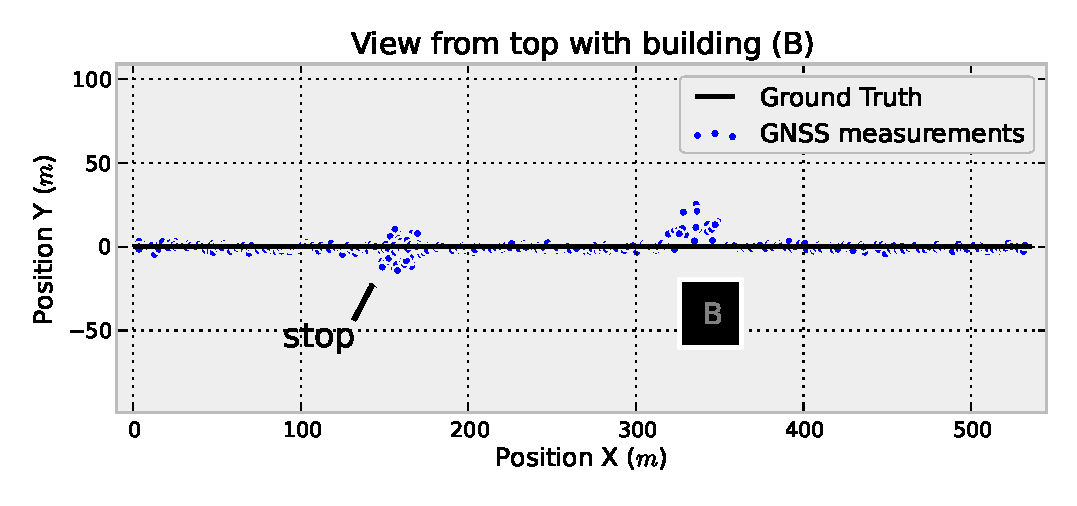
\includegraphics[width=3.0in]{images/Testdata}
\caption{Simulated GNSS measurements with vehicle stop and shading from a building (B) as well as ground truth}
\label{Testdata}
\end{figure}

The car starts at $x=0$, $y=0$ with $v=\SI{20.0}{\kilo\metre\per\hour}$ and decelerates until it stops. It is standing for $\SI{10}{\second}$ and accelerating until it reaches $v=\SI{50.0}{\kilo\metre\per\hour}$ again. Then it is passing a building, which corrupts the signal quality of the GNSS, and the position measurement is disrupted by $+\SI{15}{\metre}$ in $y$-direction.

\begin{figure}[ht]
\centering
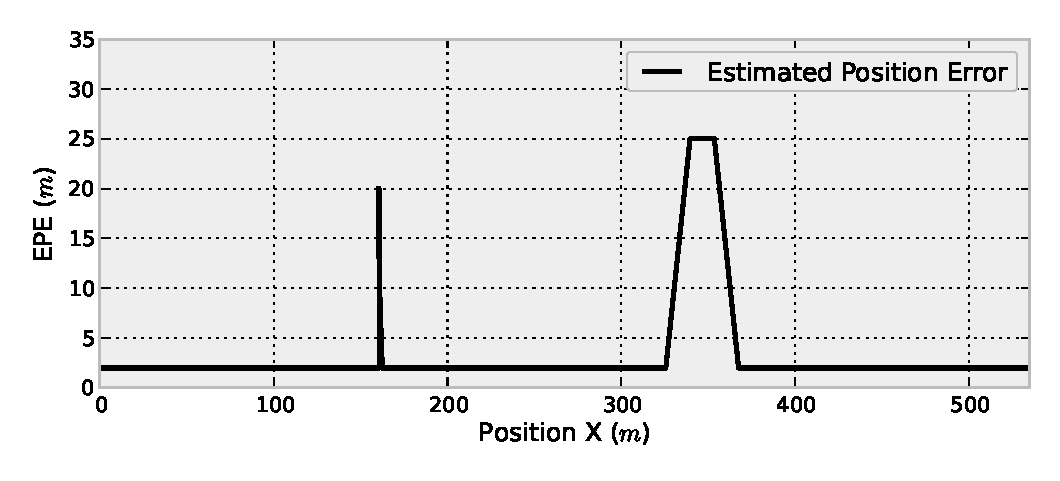
\includegraphics[width=3.0in]{images/Testdata-EPE}
\caption{Simulated GNSS Estimated Position Error}
\label{Testdata-EPE}
\end{figure}

After that, the car performs a slalom maneuvers to evaluate the dynamic capabilities of the filter.

\subsection{Parameter for Adaptive R}

The summand $\epsilon$ for \eqref{sigmav} is initialized with $\SI{0.1}{\metre\per\second}$, the exponent $\xi$ for \eqref{sigmav} with $500{,}0$ and the factor $\zeta$ for \eqref{sigmaepe} with $50{,}0$. The resulting values for $\sigma_x^2$ and $\sigma_y^2$ for a range of velocities and $EPE$s are shown in Fig. \ref{R1}.

\begin{figure}[ht]
\centering
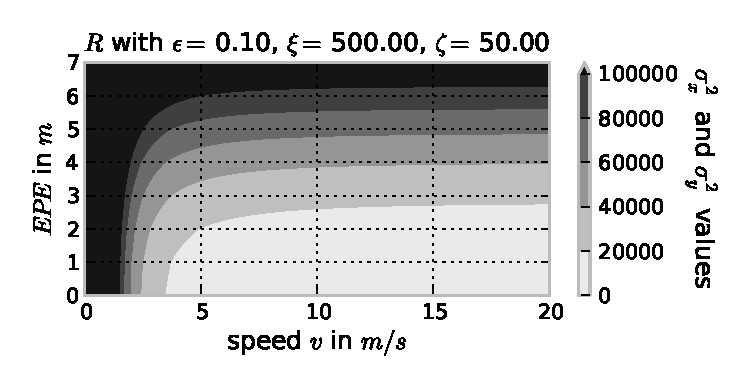
\includegraphics[width=3.0in]{images/R}
\caption{Values of $\sigma_x^2$ and $\sigma_y^2$ in $R$, depending on $v$ and $EPE$}
\label{R1}
\end{figure}

The factor $\rho$ for \eqref{sigmaroll} was initialized with $200{,}0$, the summand $\gamma$ was chosen to be $500{,}0$.

These parameters are empirically chosen and are subject to change for different cars or other driving scenarios or street qualities.

\subsection{Simulation Results}

As one can see in Fig. \ref{CTRV-Position-Testdata}, the filter follows the trajectory of the GNSS measurements. If the $EPE$ raises, the filter is more willing to trust the control input instead of the position measurements.

\begin{figure}[ht]
\centering
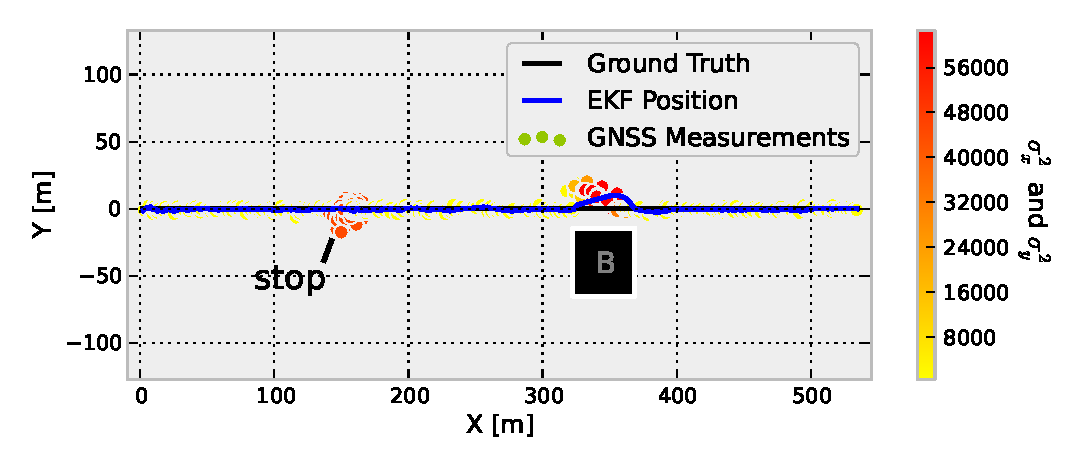
\includegraphics[width=3.0in]{images/Extended-Kalman-Filter-CTRV-Position-Testdata}
\caption{Measurements of GNSS with color coded value for $R$, depending on speed and EPE as well as estimated trajectory of the EKF}
\label{CTRV-Position-Testdata}
\end{figure}

To quantify the filter performance with respect to ground truth (GT) trajectory, the cross track error is introduced.

\begin{equation}\text{CTE}_x=x_{GT}-x\end{equation}
\begin{equation}\text{CTE}_y=y_{GT}-y\end{equation}

The sum of the square of the CTE over the whole dataset is a value to quantify the filter performance with respect to the correct trajectory estimation.

\subsection{Comparison to Standard EKF}

To compare the estimated trajectory with a non-adaptive EKF, the estimation was performed with several datasets for GNSS position measurements, generated by random Gaussian noise around the ground truth position.

The standard EKF was set up with static $\sigma_x^2=\SI{144}{\square\metre}$, $\sigma_y^2=\SI{144}{\square\metre}$ values. The result is shown in Fig.  \ref{Boxplot}.

\begin{figure}[ht]
\centering
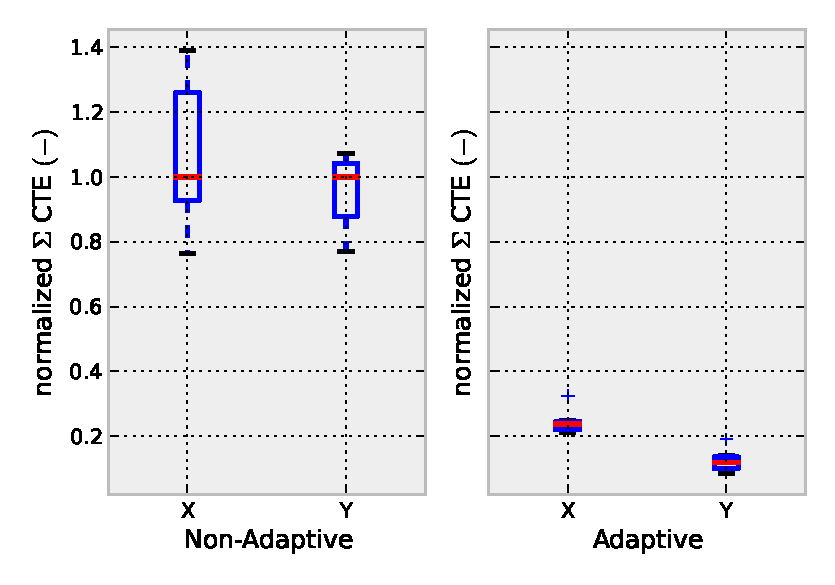
\includegraphics[width=3.0in]{images/CTE-Adaptive-NonAdaptive-Boxplot}
\caption{Comparison of the mean, upper and lower quantile of several runs for trajectory estimation and values for sum of squares of the CTE for the adaptive and the standard EKF}
\label{Boxplot}
\end{figure}

In comparison, the adaptive EKF reduces the $\Sigma \text{CTE}_{x,y}^2$ by around $\SI{80}{\percent}$, which for sure depends on the driving direction as well as on the chosen parameters.

Note, that the standard EKF could set up with high values for $R$ as well and may have better CTE values, but then, like for all filters, the dynamic is getting lost.

\section{\uppercase{Experimental Setup}}

\subsection{Low Cost Sensors}

The measurement and control data of the filter were logged by a LSM303 3-axis accelerometer and 3-axis magnetometer, ITG-3200 3-axis gyro and PA6H GNSS receiver. The sensors are available with the Tinkerforge IMU Brick and GPS Bricklet.

All sensors are mobile, so no connection to the car is neccessary, but could improve the estimation.

\subsection{Ground Truth GNSS Sensor}

The ground truth was logged with a multifrequency aerial antenna (JAVAD GrAnt-G3T) and -receiver (JAVAD Delta), corrected with a virtual reference station (VRS) and Satellite Positioning Service of the German State Survey (SAPOS) data via GPRS modem (come2ascos GenPro).

\section{\uppercase{Experimental Results}}



\begin{figure}[h!]
\centering
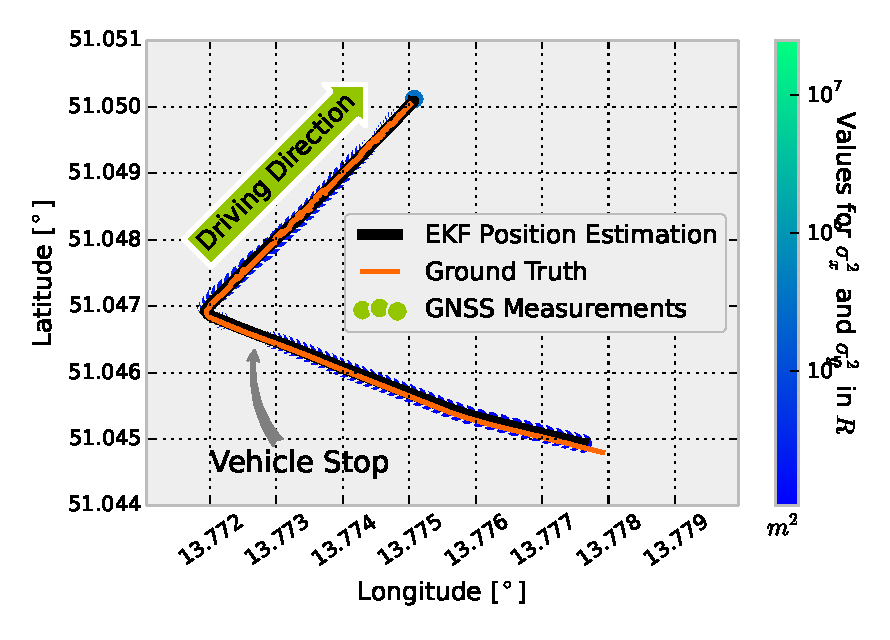
\includegraphics[width=3.0in]{images/Extended-Kalman-Filter-CTRV-Position}
\caption{Performed test drive with adaptive values of measurement uncertainty values for matrix $R$. (GNSS measurement dots are reduced to every 10th for better visualisation in this figure)}
\label{ctrv-position}
\end{figure}

The state variables $x_k$ for the scenario were estimated as shown in Fig. \ref{ctrv-states}.

\begin{figure}[ht]
\centering
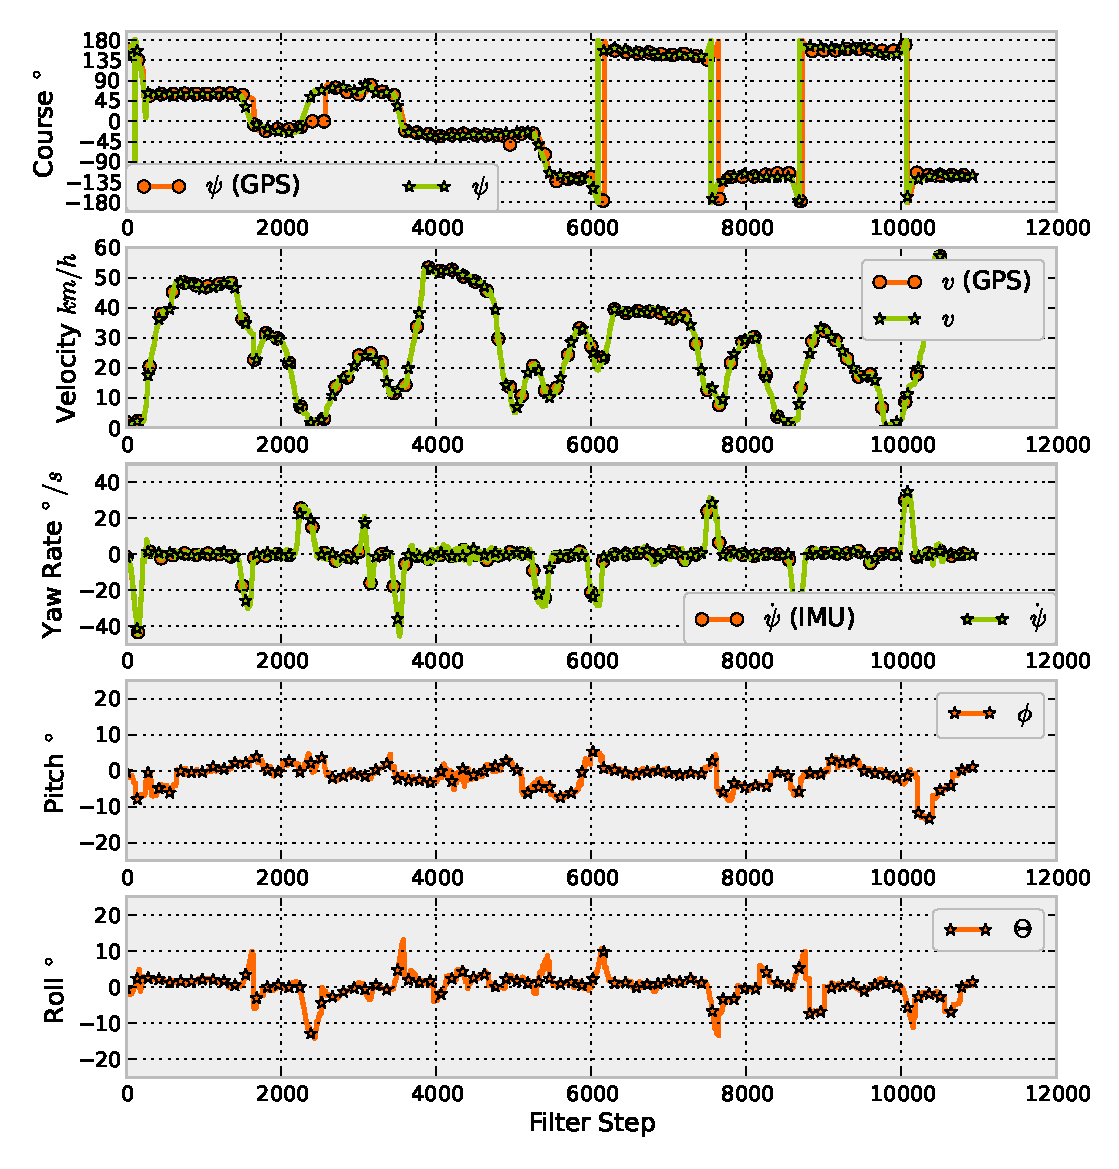
\includegraphics[width=3.0in]{images/Extended-Kalman-Filter-CTRV-Attitude-State-Estimates}
\caption{Estimated state variables $x_k$ for real world test drive}
\label{ctrv-states}
\end{figure}

As one can see, the stop before the right turn got a high position measurement uncertainty, which in detail is shown in figure \ref{ctrv-position-detail}.

\begin{figure}[ht]
\centering
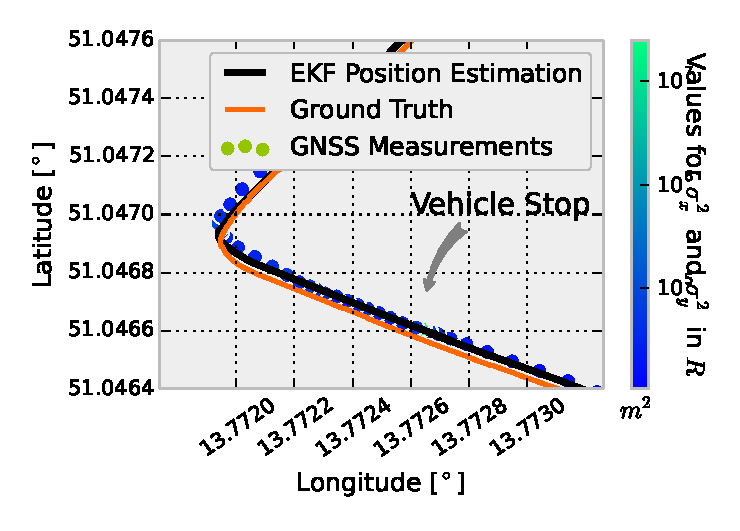
\includegraphics[width=3.0in]{images/Extended-Kalman-Filter-CTRV-Position-Detail}
\caption{Detailed view of the stop within the performed test drive with raised uncertainty for $R$. (GNSS measurement dots are reduced to every 10th for better visualisation in this figure)}
\label{ctrv-position-detail}
\end{figure}

While standing still, the heading measurement of the GNSS receiver is inaccurate (see Fig. \ref{ctrv-states} between filter step $k\approx2200\dotsc2400$). The filter performes very well on this situation and keeps the heading in the correct direction. The EKF position estimation (see Fig. \ref{ctrv-position-detail}) is not disturbed by inaccurate GNSS measurements while standing still and is dynamically responsive while cornering. The low cost GNSS equipment with the proposed adaptive Extended Kalman Filter delivers a robust position estimation, which alignes with the ground truth measurement. 

The values for the measurement uncertainties in $R$ are calculated like shown in figure \ref{adaptive-R}.

\begin{figure}[ht]
\centering
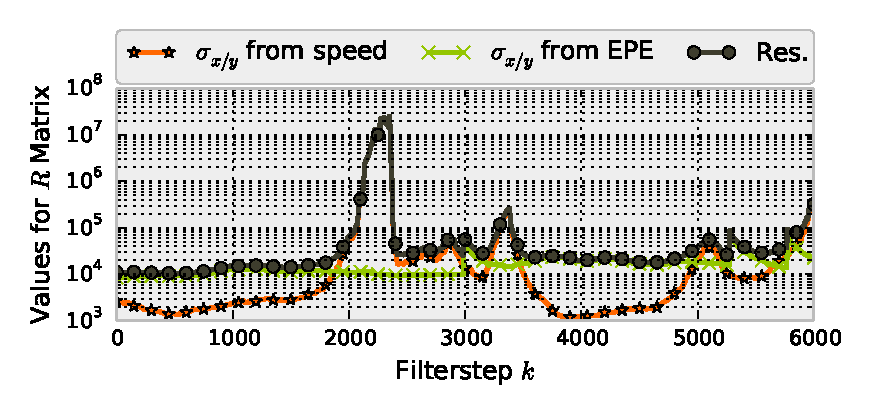
\includegraphics[width=3.0in]{images/Extended-Kalman-Filter-CTRV-Adaptive-R}
\caption{Values for adaptive $\sigma_v$, $\sigma_{EPE}$ and resulting $\sigma$ for $x$ and $y$}
\label{adaptive-R}
\end{figure}

\section{\uppercase{Conclusions}}
\label{sec:conclusion}

\noindent In this paper we presented a novel approach to adaptively calculate the measurement uncertainty for an improved position and attitude estimation, based on the Estimated Position Error and the speed, determined by the low cost GNSS receiver.
We explained the basics and used some empirically chosen values to parametrize the filter. With that, we showed with simulated data, that the filter performes significantly better than a standard Extended Kalman Filter. Based on that, we conducted test drives and used the developed Adaptive EKF for a real world dataset, which proved its ability to improve the position estimation with partly bad signal quality. In addition to that, the filter also performs pretty well on dynamic situations and is not loosing the ability to follow dynamic vehicle movements.
The filter cannot be used to get rid of bias in position estimation, because the EPE from GNSS has, by definition, no information about static drift of the position information.
The presented filter can be used to get significantly better results while standing still or driving slowly as well as keeping the heading fixed while do so.
Additionally, the attitude of the vehicle is estimated, based on the filter presented in \cite{Madgwick2010}.

\section*{\uppercase{Acknowledgements}}

\noindent The authors would like to thank the Free State of Saxony and the European Union, which funded this research from the ESF fond.


\bibliographystyle{apalike}
{\small
\bibliography{bibtex/library.bib}}


\section*{\uppercase{Appendix}}

\noindent \subsection*{Programm Code and EKF Implementation}
The implemenented EKF code as well as all figures and the data used in this paper can be found online at https://github.com/balzer82/ICINCO-2014

\subsection*{Jacobians}

The Jacobian of the state transition function \eqref{statetransitionfunction} with respect to the state $x_k$ is defined with

\begin{equation}\left[\begin{matrix}1 & 0 & J_{A,13} & J_{A,14} & 0 & 0\\0 & 1 & J_{A,23} & J_{A,24} & 0 & 0\\0 & 0 & 1 & 0 & 0 & 0\\0 & 0 & 0 & 1 & 0 & 0\\0 & 0 & 0 & 0 & 1 & 0\\0 & 0 & 0 & 0 & 0 & 1\end{matrix}\right]\end{equation}

with

\begin{equation}J_{A,13}=\frac{1}{\dot\psi} \left(- \sin{\left (\psi \right )} + \sin{\left (T \dot\psi + \psi \right )}\right)\end{equation}
\begin{equation}J_{A,14}=\frac{v}{\dot\psi} \left(- \cos{\left (\psi \right )} + \cos{\left (T \dot\psi + \psi \right )}\right)\end{equation}
\begin{equation}J_{A,23}=\frac{1}{\dot\psi} \left(\cos{\left (\psi \right )} - \cos{\left (T \dot\psi + \psi \right )}\right)\end{equation}
\begin{equation}J_{A,24}=\frac{v}{\dot\psi} \left(- \sin{\left (\psi \right )} + \sin{\left (T \dot\psi + \psi \right )}\right)\end{equation}

The Jacobian of the state transition function with respect to the control is

\begin{equation}J_G=\left[\begin{matrix}0 & J_{G,12} & 0 & 0\\0 & J_{G,22} & 0 & 0\\T & 0 & 0 & 0\\0 & T & 0 & 0\\0 & 0 & T & 0\\0 & 0 & 0 & T\end{matrix}\right]\end{equation}

with

\begin{equation}
	\begin{split}
    	J_{G,12}=\frac{T v}{\dot\psi} \cos{\left (T \dot\psi + \psi \right )} - \\ 		\frac{v}{\dot\psi^{2}} \left(- \sin{\left (\psi \right )} + \sin{\left (T \dot\psi + \psi \right )}\right)
	\end{split}
\end{equation}

\begin{equation}
	\begin{split}
    	J_{G,22}=\frac{T v}{\dot\psi} \sin{\left (T \dot\psi + \psi \right )} - \\ \frac{v}{\dot\psi^{2}} \left(\cos{\left (\psi \right )} - \cos{\left (T \dot\psi + \psi \right )}\right)
    \end{split}
\end{equation}

\vfill
\end{document}

